\chapter{Oxidação e redução}\label{ch:g11:redox}

Uma placa de zinco é mergulhada numa solução azul de sulfato de cobre. Em
poucos minutos, a sua superfície escurece sob uma camada esponjosa,
castanho-avermelhada; uma hora depois, o azul da solução desbotou.
Apareceu cobre metálico onde não havia nenhum, e o zinco passou para a
solução na forma de \omterm{def:g9:ions:ion}{íons} invisíveis. Nada foi aquecido, nenhum gás foi
liberado, nenhum oxigênio participou --- e, mesmo assim, os químicos
chamam isso de \omterm{def:g11:redox:oxidation}{oxidação}. A palavra queria dizer ``combinar-se com o
oxigênio''; hoje ela quer dizer uma coisa mais geral e mais útil: a
perda de \omterm{def:g9:inside-the-atom:nucleus}{elétrons}. Este capítulo acompanha os \omterm{def:g9:inside-the-atom:nucleus}{elétrons}.

\begin{recall}
Um \omterm{def:g9:ions:ion}{íon} é um \omterm{def:g7:atoms-and-molecules:atom}{átomo} ou um grupo de \omterm{def:g7:atoms-and-molecules:atom}{átomos} que ganhou ou perdeu \omterm{def:g9:inside-the-atom:nucleus}{elétrons}
(\cref{ch:g9:ions}). Um \omterm{def:g9:periodic-table-first-look:metal}{metal} como o ferro ou o zinco reage com o ácido
clorídrico e dá hidrogênio e \omterm{def:g9:ions:ion}{íons} metálicos
(\cref{ch:g9:metals-acids-corrosion}). Uma \omterm{def:g10:the-mole:amount}{quantidade de matéria} $n$, em
\omterm{def:g10:the-mole:amount}{mols}, é calculada a partir de uma massa $m$ por $n = m/M$
(\cref{ch:g10:the-mole}).
\end{recall}

\begin{omfigure}
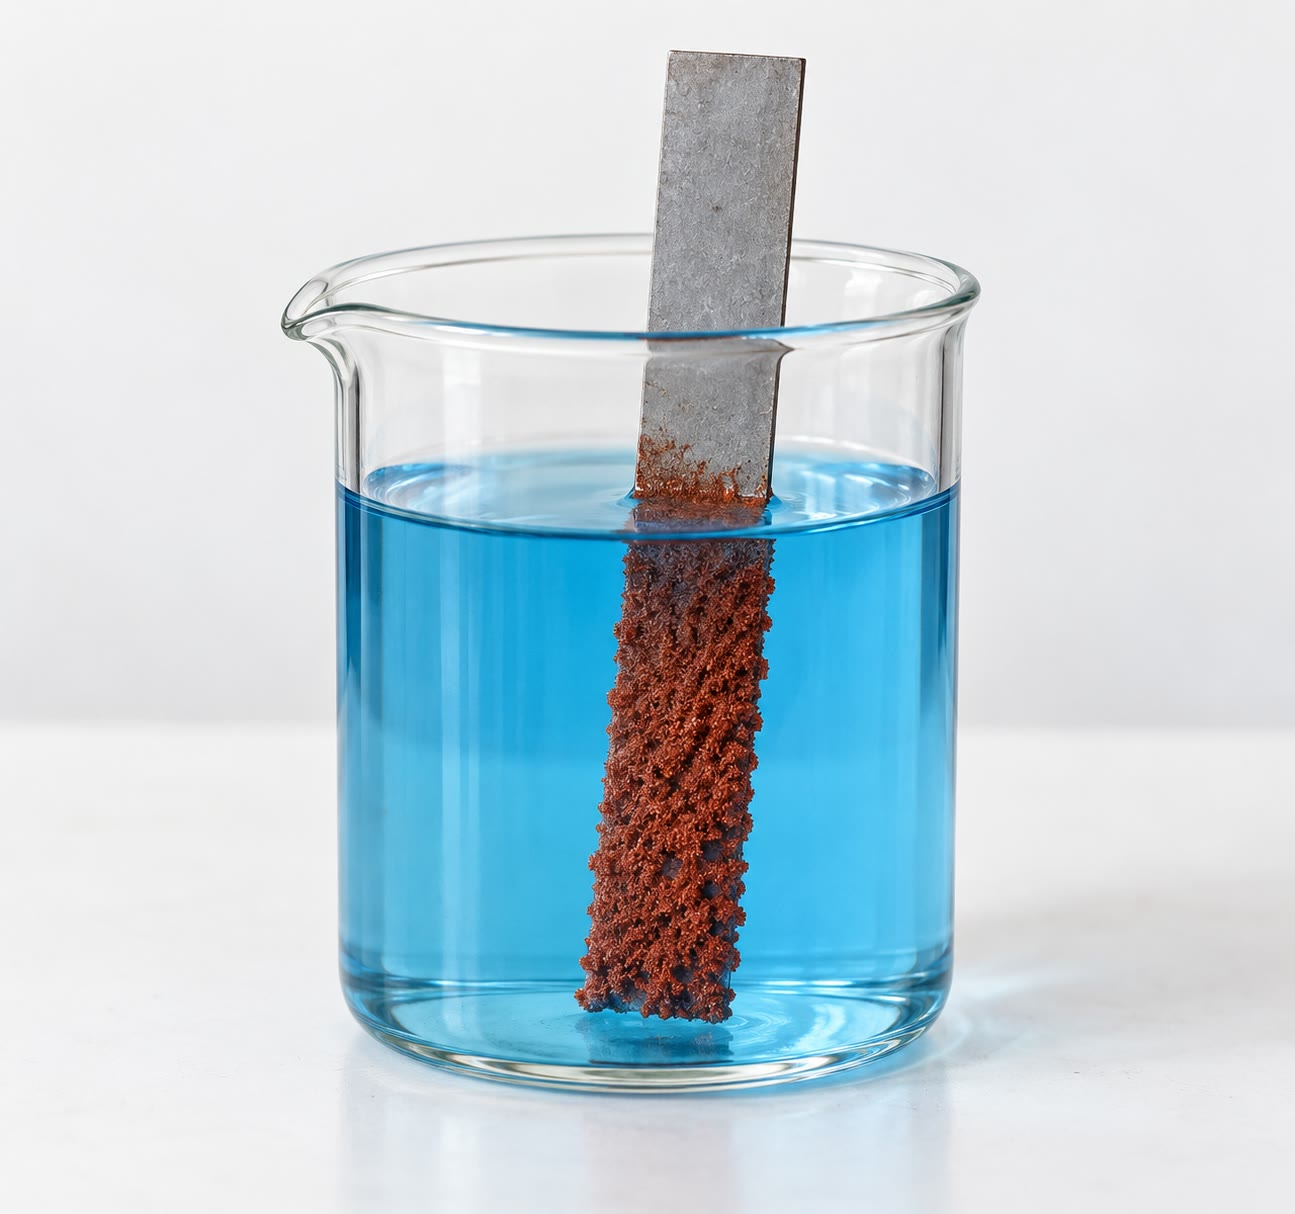
\includegraphics[width=0.55\linewidth]{images/book1/ai/g11-zinc-copper-sulfate.jpg}

{\small Uma placa de zinco numa solução de sulfato de cobre: o cobre se
deposita sobre o zinco, e os \omterm{def:g9:ions:ion}{íons} zinco tomam o seu lugar na solução.}
\end{omfigure}

\section{Oxidantes e redutores}

\begin{definition}[Oxidante e redutor]\label{def:g11:redox:oxidant}
Um \emph{oxidante}\index{oxidante} é uma espécie capaz de ganhar um ou
mais \omterm{def:g9:inside-the-atom:nucleus}{elétrons}. Um \emph{redutor}\index{redutor} é uma espécie capaz de
ceder um ou mais \omterm{def:g9:inside-the-atom:nucleus}{elétrons}.
\end{definition}

\begin{definition}[Oxidação e redução]\label{def:g11:redox:oxidation}
Uma \emph{oxidação}\index{oxidacao@oxidação} é uma perda de \omterm{def:g9:inside-the-atom:nucleus}{elétrons}; uma
\emph{redução}\index{reducao@redução} é um ganho de \omterm{def:g9:inside-the-atom:nucleus}{elétrons}. Um \omterm{def:g11:redox:oxidant}{redutor} é
oxidado; um \omterm{def:g11:redox:oxidant}{oxidante} é reduzido.
\end{definition}

\begin{remark}[Um jeito de lembrar]\label{rem:g11:redox:remember}
Na \emph{\omterm{def:g11:redox:oxidation}{redução}}, a carga da espécie é reduzida: \ce{Cu^{2+}}, ganhando
dois \omterm{def:g9:inside-the-atom:nucleus}{elétrons}, vira \ce{Cu}, carga $+2 \to 0$. Numa \omterm{def:g11:redox:oxidation}{oxidação}, a carga
sobe: \ce{Zn -> Zn^{2+} + 2e-}, $0 \to +2$.
\end{remark}

\begin{definition}[Par redox e semirreação]\label{def:g11:redox:couple}
Um \omterm{def:g11:redox:oxidant}{oxidante} e o \omterm{def:g11:redox:oxidant}{redutor} em que ele se transforma ganhando \omterm{def:g9:inside-the-atom:nucleus}{elétrons}
formam um \emph{par redox}\index{par redox}, escrito Ox/Red com o
\omterm{def:g11:redox:oxidant}{oxidante} primeiro: \ce{Cu^{2+}}/\ce{Cu}, \ce{Zn^{2+}}/\ce{Zn}. A troca de
\omterm{def:g9:inside-the-atom:nucleus}{elétrons} dentro de um par é descrita pela sua
\emph{semirreação}\index{semirreacao@semirreação},
\[
  \text{Ox} + n\,\ce{e-} \ce{<=>} \text{Red}, % ce-unbalanced-ok (generic form)
\]
balanceada em \omterm{def:g7:atoms-and-molecules:atom}{átomos} e em carga, por exemplo
$\ce{Cu^{2+}(aq) + 2e- <=> Cu(s)}$. A seta dupla diz que a troca pode
acontecer nos dois sentidos.
\end{definition}

\begin{example}[Os metais e os seus íons]\label{ex:g11:redox:metals}
Cada \omterm{def:g9:periodic-table-first-look:metal}{metal} forma um par com o seu \omterm{def:g9:ions:ion}{íon}:
\begin{center}
\begin{tabular}{ll}
\hline
par & \omterm{def:g11:redox:couple}{semirreação} \\
\hline
\ce{Ag+}/\ce{Ag} & \ce{Ag+ + e- <=> Ag} \\
\ce{Cu^{2+}}/\ce{Cu} & \ce{Cu^{2+} + 2e- <=> Cu} \\
\ce{Fe^{2+}}/\ce{Fe} & \ce{Fe^{2+} + 2e- <=> Fe} \\
\ce{Zn^{2+}}/\ce{Zn} & \ce{Zn^{2+} + 2e- <=> Zn} \\
\ce{Al^{3+}}/\ce{Al} & \ce{Al^{3+} + 3e- <=> Al} \\
\hline
\end{tabular}
\end{center}
Os \omterm{def:g9:ions:ion}{íons} também podem formar pares: \ce{Fe^{3+} + e- <=> Fe^{2+}} para o
par \ce{Fe^{3+}}/\ce{Fe^{2+}}, e \ce{I2 + 2e- <=> 2I-} para
\ce{I2}/\ce{I-}. O hidrogênio também: \ce{2H+ + 2e- <=> H2} para
\ce{H+}/\ce{H2}.
\end{example}

\begin{remark}[Uma espécie, dois papéis]\label{rem:g11:redox:amphoteric}
Uma espécie pode ser o \omterm{def:g11:redox:oxidant}{redutor} de um par e o \omterm{def:g11:redox:oxidant}{oxidante} de outro. O \omterm{def:g9:ions:ion}{íon}
\ce{Fe^{2+}} é o \omterm{def:g11:redox:oxidant}{oxidante} de \ce{Fe^{2+}}/\ce{Fe} e o \omterm{def:g11:redox:oxidant}{redutor} de
\ce{Fe^{3+}}/\ce{Fe^{2+}}. O papel que ele desempenha depende do seu
parceiro na reação.
\end{remark}

\section{As reações de oxirredução}

\begin{definition}[Reação de oxirredução]\label{def:g11:redox:reaction}
Uma \emph{reação de oxirredução}\index{reacao de oxirreducao@reação de oxirredução} é uma
transferência de \omterm{def:g9:inside-the-atom:nucleus}{elétrons} do \omterm{def:g11:redox:oxidant}{redutor} de um par para o \omterm{def:g11:redox:oxidant}{oxidante} de outro.
O \omterm{def:g11:redox:oxidant}{redutor} é oxidado e o \omterm{def:g11:redox:oxidant}{oxidante} é reduzido, ao mesmo tempo.
\end{definition}

\begin{proposition}[Nenhum elétron livre]\label{prop:g11:redox:no-free-electrons}
Os \omterm{def:g9:inside-the-atom:nucleus}{elétrons} não existem livres numa solução: cada \omterm{def:g9:inside-the-atom:nucleus}{elétron} cedido pelo
\omterm{def:g11:redox:oxidant}{redutor} é tomado pelo \omterm{def:g11:redox:oxidant}{oxidante}. A equação de uma \omterm{def:g11:redox:reaction}{reação de oxirredução} é
obtida, portanto, somando as duas \omterm{def:g11:redox:couple}{semirreações}, cada uma multiplicada
pelo número que torna os \omterm{def:g9:inside-the-atom:nucleus}{elétrons} cedidos iguais aos \omterm{def:g9:inside-the-atom:nucleus}{elétrons} tomados;
os \omterm{def:g9:inside-the-atom:nucleus}{elétrons} se cancelam então e não aparecem na equação.
\end{proposition}

\begin{example}[O zinco e os íons cobre]\label{ex:g11:redox:zinc-copper}
Na cena de abertura, o zinco é oxidado e os \omterm{def:g9:ions:ion}{íons} cobre são reduzidos:
\[
\begin{array}{l@{\qquad}l}
  \ce{Zn(s) -> Zn^{2+}(aq) + 2e-} & \text{(oxidação)}\\
  \ce{Cu^{2+}(aq) + 2e- -> Cu(s)} & \text{(redução)}\\
  \hline
  \ce{Zn(s) + Cu^{2+}(aq) -> Zn^{2+}(aq) + Cu(s)} &
\end{array}
\]
Dois \omterm{def:g9:inside-the-atom:nucleus}{elétrons} passam de cada \omterm{def:g7:atoms-and-molecules:atom}{átomo} de zinco para um \omterm{def:g9:ions:ion}{íon} cobre. A cor azul
da solução é a cor dos \omterm{def:g9:ions:ion}{íons} \ce{Cu^{2+}}; ela desbota à medida que eles
são consumidos, enquanto os \omterm{def:g9:ions:ion}{íons} \ce{Zn^{2+}}, incolores, tomam o seu
lugar.
\end{example}

\begin{omfigure}
\begin{tikzpicture}[font=\small, >=Stealth,
    ion/.style={circle, draw=black!70, minimum size=10mm, inner sep=0pt}]
  % the zinc strip and the solution
  \fill[black!18] (0,0) rectangle (1.6,4);
  \draw[black!60] (1.6,0) -- (1.6,4);
  \node[anchor=south] at (0.8,0.08) {zinco};
  \fill[omWater!60] (1.6,0) rectangle (9.0,4);
  \node[anchor=north east] at (8.95,3.95) {solução};
  % a zinc atom leaves as an ion
  \node[ion, fill=black!30] (zn) at (1.15,3.0) {\ce{Zn}};
  \node[ion, fill=white] (znion) at (5.0,3.0) {\ce{Zn^{2+}}};
  \draw[->, thick, omProp] (zn.east) -- (znion.west)
    node[midway, above] {oxidação};
  % the electrons travel through the metal
  \draw[->, thick, omDef, dashed] (0.75,2.45) -- (0.75,1.55)
    node[midway, right] {2\,\ce{e-}};
  % a copper ion is reduced on the surface
  \node[ion, fill=omDef!35] (cuion) at (5.0,1.0) {\ce{Cu^{2+}}};
  \node[ion, fill=orange!55!brown] (cu) at (2.12,1.0) {\ce{Cu}};
  \draw[->, thick, omProp] (cuion.west) -- (cu.east)
    node[midway, above] {redução};
  \node[anchor=west, align=left] at (6.1,2.0) {cada átomo de zinco dá\\ dois elétrons a um\\ íon cobre};
\end{tikzpicture}

{\small Na superfície do zinco. Um \omterm{def:g7:atoms-and-molecules:atom}{átomo} de zinco perde dois \omterm{def:g9:inside-the-atom:nucleus}{elétrons} e
sai como um \omterm{def:g9:ions:ion}{íon} \ce{Zn^{2+}}; os dois \omterm{def:g9:inside-the-atom:nucleus}{elétrons} atravessam o \omterm{def:g9:periodic-table-first-look:metal}{metal} até um
\omterm{def:g9:ions:ion}{íon} \ce{Cu^{2+}} que toca a superfície, que vira um \omterm{def:g7:atoms-and-molecules:atom}{átomo} de cobre e
fica na placa.}
\end{omfigure}

\begin{omfigure}
\begin{tikzpicture}[font=\small]
  \pic at (0,0) {beaker={0.75}{omDef!45}};
  \fill[black!35] (-0.15,0.25) rectangle (0.15,2.5);
  \draw[black!65] (-0.15,0.25) rectangle (0.15,2.5);
  \node[anchor=north, align=center] at (0,-0.15) {no início:\\ solução azul de \ce{Cu^{2+}}};
  \draw[->, thick, omProp] (1.3,1) -- (3.2,1) node[midway, above] {uma hora};
  \pic at (4.5,0) {beaker={0.75}{omDef!12}};
  \fill[black!35] (4.35,0.25) rectangle (4.65,2.5);
  \fill[orange!55!brown] (4.3,0.25) rectangle (4.7,1.5);
  \draw[black!65] (4.35,0.25) rectangle (4.65,2.5);
  \node[anchor=north, align=center] at (4.5,-0.15) {depois: solução mais clara,\\ cobre sobre o zinco};
\end{tikzpicture}

{\small O que se vê: o depósito de cobre na parte mergulhada da placa, e
o desbotamento da cor azul dos \omterm{def:g9:ions:ion}{íons} \ce{Cu^{2+}}.}
\end{omfigure}

\begin{example}[Os metais no ácido, de novo]\label{ex:g11:redox:acid}
Quando o ferro \omterm{def:g2:mixing-and-dissolving:dissolve}{se dissolve} no ácido clorídrico, o ferro é oxidado e os
\omterm{def:g9:ions:ion}{íons} \ce{H+} são reduzidos a hidrogênio:
\[
  \ce{Fe(s) + 2H+(aq) -> Fe^{2+}(aq) + H2(g)}.
\]
Os pares são \ce{Fe^{2+}}/\ce{Fe} e \ce{H+}/\ce{H2}; os \omterm{def:g9:ions:ion}{íons} cloreto não
participam.
\end{example}

\begin{inthelab}[A árvore de prata]
Uma espiral de fio de cobre limpo é pendurada num béquer com uma solução
diluída de nitrato de prata, \ce{Ag+(aq) + NO3^-(aq)}. Em menos de uma
hora, agulhas ramificadas de prata brilhante crescem ao longo do fio, e
a solução incolor fica azul-clara:
\ce{Cu(s) + 2Ag+(aq) -> Cu^{2+}(aq) + 2Ag(s)}. O experimento é feito
pelo professor, com luvas e óculos de proteção, e a solução é depois
recolhida como resíduo perigoso.
\end{inthelab}

\begin{safety}{\ghs[0.82cm]{GHS03}\ghs[0.82cm]{GHS05}\ghs[0.82cm]{GHS08}\ghs[0.82cm]{GHS09}}
% ledger: ghs:AgNO3
Nitrato de prata: um \omterm{def:g11:redox:oxidant}{oxidante} que pode alimentar um incêndio (GHS03);
corrosivo para a pele e os olhos, e mancha a pele de preto (GHS05); um
perigo para a saúde (GHS08); muito tóxico para os organismos aquáticos,
por isso nunca vai para a pia (GHS09).
\end{safety}

\begin{omfigure}
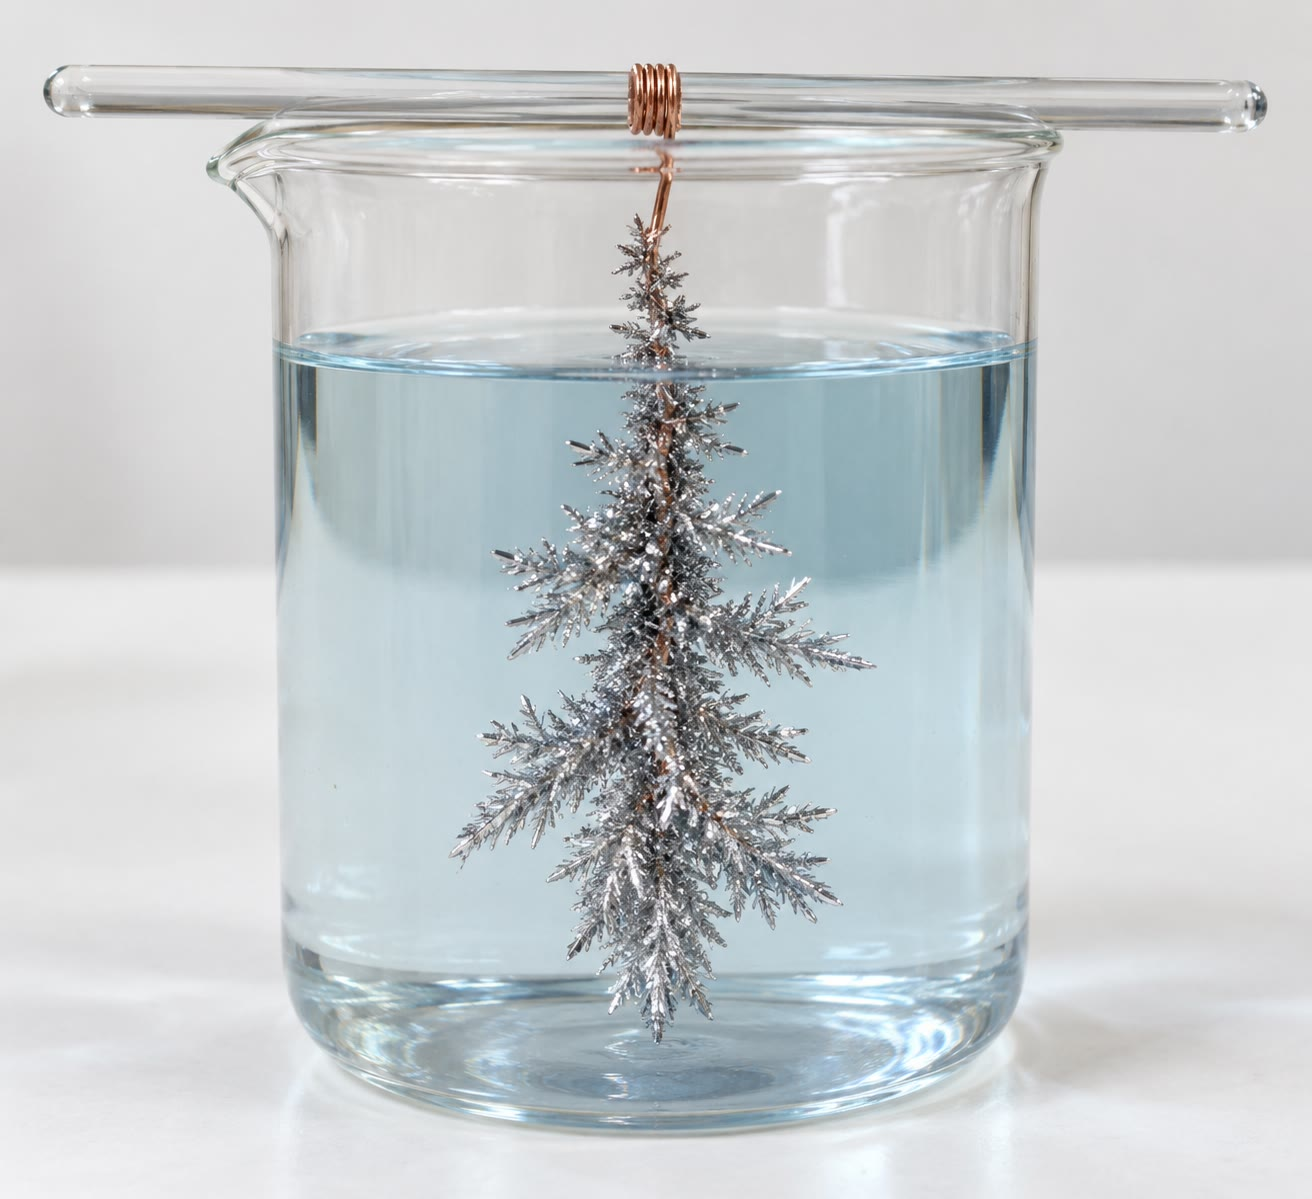
\includegraphics[width=0.5\linewidth]{images/book1/ai/g11-silver-tree.jpg}

{\small Cristais de prata crescendo num fio de cobre numa solução de
nitrato de prata.}
\end{omfigure}

\section{Balancear semirreações}

Muitos pares importantes contêm oxigênio e são escritos para \omterm{def:g9:acids-bases-ph:acidic}{soluções
ácidas}, em que há \omterm{def:g9:ions:ion}{íons} \ce{H+}. As suas \omterm{def:g11:redox:couple}{semirreações} precisam de
\omterm{def:g7:atoms-and-molecules:molecule}{moléculas} de água e de \omterm{def:g9:ions:ion}{íons} \ce{H+} para ser balanceadas.

\begin{method}[Balancear uma semirreação em solução ácida]\label{met:g11:redox:balance}
Para escrever a \omterm{def:g11:redox:couple}{semirreação} de um par Ox/Red em \omterm{def:g9:acids-bases-ph:acidic}{solução ácida}:
\begin{enumerate}
  \item escreva Ox à esquerda e Red à direita, e balanceie o \omterm{def:g7:atoms-and-molecules:atom}{átomo} que
        não é nem O nem H;
  \item balanceie os \omterm{def:g7:atoms-and-molecules:atom}{átomos} de oxigênio com \omterm{def:g7:atoms-and-molecules:molecule}{moléculas} de água \ce{H2O};
  \item balanceie os \omterm{def:g7:atoms-and-molecules:atom}{átomos} de hidrogênio com \omterm{def:g9:ions:ion}{íons} \ce{H+};
  \item balanceie a carga com \omterm{def:g9:inside-the-atom:nucleus}{elétrons} \ce{e-}, à esquerda;
  \item verifique: o mesmo número de cada \omterm{def:g7:atoms-and-molecules:atom}{átomo} e a mesma carga total
        dos dois lados.
\end{enumerate}
\end{method}

\begin{example}[O íon permanganato]\label{ex:g11:redox:permanganate}
Para o par \ce{MnO4^-}/\ce{Mn^{2+}} (de violeta intenso a quase incolor):
o manganês está balanceado; quatro O à esquerda dão $\ce{4H2O}$ à
direita; os seus oito H dão $\ce{8H+}$ à esquerda; a carga à esquerda é
$-1 + 8 = +7$, à direita $+2$, por isso acrescentam-se cinco \omterm{def:g9:inside-the-atom:nucleus}{elétrons} à
esquerda:
\[
  \ce{MnO4^-(aq) + 8H+(aq) + 5e- <=> Mn^{2+}(aq) + 4H2O(l)}.
\]
\end{example}

\begin{example}[O íon dicromato]\label{ex:g11:redox:dichromate}
Para \ce{Cr2O7^{2-}}/\ce{Cr^{3+}} (de laranja a verde): dois cromos à
direita; sete O dão \ce{7H2O}; catorze H dão \ce{14H+}; carga
$-2 + 14 = +12$ à esquerda contra $2 \times 3 = +6$ à direita, logo seis
\omterm{def:g9:inside-the-atom:nucleus}{elétrons}:
\[
  \ce{Cr2O7^{2-}(aq) + 14H+(aq) + 6e- <=> 2Cr^{3+}(aq) + 7H2O(l)}.
\]
\end{example}

\begin{method}[Escrever uma equação de oxirredução]\label{met:g11:redox:combine}
Para escrever a equação da reação entre o \omterm{def:g11:redox:oxidant}{oxidante} Ox$_1$ de um par e o
\omterm{def:g11:redox:oxidant}{redutor} Red$_2$ de outro:
\begin{enumerate}
  \item escreva as duas \omterm{def:g11:redox:couple}{semirreações}, a primeira no sentido da \omterm{def:g11:redox:oxidation}{redução}
        (Ox$_1 \to$ Red$_1$), a segunda no sentido da \omterm{def:g11:redox:oxidation}{oxidação}
        (Red$_2 \to$ Ox$_2$);
  \item multiplique-as pelos menores números que igualam os \omterm{def:g9:inside-the-atom:nucleus}{elétrons};
  \item some-as; os \omterm{def:g9:inside-the-atom:nucleus}{elétrons} se cancelam, e talvez também alguns
        \ce{H+} e \ce{H2O} que aparecem dos dois lados;
  \item verifique mais uma vez os \omterm{def:g7:atoms-and-molecules:atom}{átomos} e a carga.
\end{enumerate}
\end{method}

\begin{example}[O permanganato e o ferro(II)]\label{ex:g11:redox:mno4-fe}
O \omterm{def:g9:ions:ion}{íon} permanganato oxida os \omterm{def:g9:ions:ion}{íons} \ce{Fe^{2+}} a \ce{Fe^{3+}}:
\[
\begin{array}{l@{\qquad}l}
  \ce{MnO4^- + 8H+ + 5e- -> Mn^{2+} + 4H2O} & \times 1\\
  \ce{Fe^{2+} -> Fe^{3+} + e-} & \times 5\\
  \hline
  \ce{MnO4^- + 8H+ + 5Fe^{2+} -> Mn^{2+} + 5Fe^{3+} + 4H2O} &
\end{array}
\]
Carga à esquerda: $-1 + 8 + 10 = +17$; à direita: $2 + 15 = +17$. Essa
reação é usada no próximo capítulo para medir uma quantidade de
ferro(II).
\end{example}

\section{Oxidantes e redutores à nossa volta}

\begin{proposition}[Alguns oxidantes e redutores comuns]\label{prop:g11:redox:common}
As espécies seguintes aparecem o tempo todo no laboratório e na vida
cotidiana:
\begin{center}
\small
\begin{tabular}{lll}
\hline
espécie & papel & \omterm{def:g11:redox:couple}{semirreação} do seu par \\
\hline
gás oxigênio \ce{O2} & \omterm{def:g11:redox:oxidant}{oxidante} & \ce{O2 + 4H+ + 4e- <=> 2H2O} \\
gás cloro \ce{Cl2} & \omterm{def:g11:redox:oxidant}{oxidante} & \ce{Cl2 + 2e- <=> 2Cl-} \\
hipoclorito \ce{ClO-} (água sanitária) & \omterm{def:g11:redox:oxidant}{oxidante} & \ce{2ClO- + 4H+ + 2e- <=> Cl2 + 2H2O} \\
peróxido de hidrogênio \ce{H2O2} & \omterm{def:g11:redox:oxidant}{oxidante} & \ce{H2O2 + 2H+ + 2e- <=> 2H2O} \\
permanganato \ce{MnO4^-} & \omterm{def:g11:redox:oxidant}{oxidante} & \ce{MnO4^- + 8H+ + 5e- <=> Mn^{2+} + 4H2O} \\
\omterm{def:g9:periodic-table-first-look:metal}{metais} \ce{M} (\ce{Fe}, \ce{Zn}, \ce{Al}\dots) & \omterm{def:g11:redox:oxidant}{redutores} & \ce{M^{n+} + $n$ e- <=> M} % ce-unbalanced-ok (generic)
\\
iodeto \ce{I-} & \omterm{def:g11:redox:oxidant}{redutor} & \ce{I2 + 2e- <=> 2I-} \\
tiossulfato \ce{S2O3^{2-}} & \omterm{def:g11:redox:oxidant}{redutor} & \ce{S4O6^{2-} + 2e- <=> 2S2O3^{2-}} \\
ácido ascórbico \ce{C6H8O6} (vitamina C) & \omterm{def:g11:redox:oxidant}{redutor} & \ce{C6H6O6 + 2H+ + 2e- <=> C6H8O6} \\
\hline
\end{tabular}
\end{center}
\end{proposition}

\begin{example}[O cobre fica verde]\label{ex:g11:redox:patina}
Os telhados e as estátuas de cobre, deixados ao \omterm{def:g4:air-a-mixture-of-gases:air}{ar} livre durante décadas,
vão ficando verde-claros. O oxigênio do \omterm{def:g4:air-a-mixture-of-gases:air}{ar} oxida o cobre a \omterm{def:g9:ions:ion}{íons}
\ce{Cu^{2+}}, que, com a água e o dióxido de carbono, formam uma fina
crosta verde, a pátina. Ao contrário da \omterm{def:g9:metals-acids-corrosion:corrosion}{ferrugem} do ferro, a pátina gruda
no \omterm{def:g9:periodic-table-first-look:metal}{metal} e o protege de novos ataques.
\end{example}

\begin{omfigure}

\includegraphics[width=0.48\linewidth]{images/book1/ai/g11-green-roof.jpg}

{\small Um telhado de cobre depois de décadas ao \omterm{def:g4:air-a-mixture-of-gases:air}{ar}: o cobre oxidado
forma uma pátina verde.}
\end{omfigure}

\begin{remark}[Antioxidantes]\label{rem:g11:redox:antioxidant}
Um ``antioxidante'' acrescentado aos alimentos é um \omterm{def:g11:redox:oxidant}{redutor} que é oxidado
pelo oxigênio do \omterm{def:g4:air-a-mixture-of-gases:air}{ar} antes do alimento. A vitamina C (ácido ascórbico) é o
mais comum: uma maçã cortada regada com suco de limão escurece muito mais
devagar, porque a vitamina C do limão é oxidada primeiro.
\end{remark}

\section{Exercícios}

\begin{exercise}[$\star$]\label{exo:g11:redox:1}
Defina um \omterm{def:g11:redox:oxidant}{oxidante}, um \omterm{def:g11:redox:oxidant}{redutor}, uma \omterm{def:g11:redox:oxidation}{oxidação} e uma \omterm{def:g11:redox:oxidation}{redução}.
\end{exercise}

\begin{exercise}[$\star$]\label{exo:g11:redox:2}
Para cada dupla, escreva o \omterm{def:g11:redox:couple}{par redox} na forma Ox/Red: \ce{Fe} e
\ce{Fe^{2+}}; \ce{Ag} e \ce{Ag+}; \ce{I-} e \ce{I2}; \ce{Fe^{2+}} e
\ce{Fe^{3+}}.
\end{exercise}

\begin{exercise}[$\star$]\label{exo:g11:redox:3}
Escreva as \omterm{def:g11:redox:couple}{semirreações} dos pares \ce{Ag+}/\ce{Ag},
\ce{Al^{3+}}/\ce{Al}, \ce{Fe^{3+}}/\ce{Fe^{2+}} e \ce{Cl2}/\ce{Cl-}.
\end{exercise}

\begin{exercise}[$\star$]\label{exo:g11:redox:4}
A transformação \ce{Fe -> Fe^{2+} + 2e-} é uma \omterm{def:g11:redox:oxidation}{oxidação} ou uma \omterm{def:g11:redox:oxidation}{redução}?
O ferro age como \omterm{def:g11:redox:oxidant}{oxidante} ou como \omterm{def:g11:redox:oxidant}{redutor}?
\end{exercise}

\begin{exercise}[$\star$]\label{exo:g11:redox:5}
Na reação \ce{Zn + Cu^{2+} -> Zn^{2+} + Cu}, dê o nome da espécie
oxidada, da espécie reduzida, do \omterm{def:g11:redox:oxidant}{oxidante} e do \omterm{def:g11:redox:oxidant}{redutor}, e dê o número de
\omterm{def:g9:inside-the-atom:nucleus}{elétrons} transferidos para cada \omterm{def:g7:atoms-and-molecules:atom}{átomo} de zinco.
\end{exercise}

\begin{exercise}[$\star\star$]\label{exo:g11:redox:6}
Balanceie, em \omterm{def:g9:acids-bases-ph:acidic}{solução ácida}, a \omterm{def:g11:redox:couple}{semirreação} do par \ce{H2O2}/\ce{H2O},
seguindo o \cref{met:g11:redox:balance} passo a passo.
\end{exercise}

\begin{exercise}[$\star\star$]\label{exo:g11:redox:7}
Escreva a equação da reação entre o iodo \ce{I2} e o \omterm{def:g9:ions:ion}{íon} tiossulfato
\ce{S2O3^{2-}}, que dá \omterm{def:g9:ions:ion}{íons} iodeto e \omterm{def:g9:ions:ion}{íons} tetrationato \ce{S4O6^{2-}}.
\end{exercise}

\begin{exercise}[$\star\star$]\label{exo:g11:redox:8}
Escreva a equação da reação da árvore de prata a partir das suas duas
\omterm{def:g11:redox:couple}{semirreações}, e explique por que a solução fica azul.
\end{exercise}

\begin{exercise}[$\star\star$]\label{exo:g11:redox:9}
A vitamina C, \ce{C6H8O6}, reage com o iodo \ce{I2}. Escreva a equação
da reação, e diga qual espécie é o \omterm{def:g11:redox:oxidant}{redutor}.
\end{exercise}

\begin{exercise}[$\star\star$]\label{exo:g11:redox:10}
O alumínio reage com os \omterm{def:g9:ions:ion}{íons} cobre(II). Escreva a equação, e explique
por que as \omterm{def:g11:redox:couple}{semirreações} devem ser multiplicadas por 2 e por 3.
\end{exercise}

\begin{exercise}[$\star\star$]\label{exo:g11:redox:11}
O peróxido de hidrogênio oxida os \omterm{def:g9:ions:ion}{íons} ferro(II) a \omterm{def:g9:ions:ion}{íons} ferro(III) em
\omterm{def:g9:acids-bases-ph:acidic}{solução ácida}. Escreva a equação.
\end{exercise}

\begin{exercise}[$\star\star\star$]\label{exo:g11:redox:12}
Uma placa de zinco perde \qty{1.30}{g} numa solução que contém um
excesso de \omterm{def:g9:ions:ion}{íons} cobre(II). Que massa de cobre se deposita? Tome
$M(\ce{Zn}) = \qty{65.4}{g/mol}$ e $M(\ce{Cu}) = \qty{63.5}{g/mol}$.
\end{exercise}

\begin{exercise}[$\star\star\star$]\label{exo:g11:redox:13}
Escreva a equação da \omterm{def:g11:redox:oxidation}{oxidação} dos \omterm{def:g9:ions:ion}{íons} ferro(II) pelos \omterm{def:g9:ions:ion}{íons} dicromato em
\omterm{def:g9:acids-bases-ph:acidic}{solução ácida}. Que quantidade de \ce{Fe^{2+}} é oxidada por
\qty{0.010}{mol} de \omterm{def:g9:ions:ion}{íons} dicromato?
\end{exercise}

\begin{exercise}[$\star\star\star$]\label{exo:g11:redox:14}
A água sanitária contém \omterm{def:g9:ions:ion}{íons} hipoclorito \ce{ClO-} e \omterm{def:g9:ions:ion}{íons} cloreto
\ce{Cl-}. Usando os pares \ce{ClO-}/\ce{Cl2} e \ce{Cl2}/\ce{Cl-},
escreva a equação da reação que acontece quando a água sanitária
encontra um ácido, e explique por que os rótulos da água sanitária e dos
removedores de calcário ácidos avisam, os dois, para nunca misturá-los.
\end{exercise}

\begin{exercise}[$\star\star\star$]\label{exo:g11:redox:15}
Na figura da superfície do zinco, os \omterm{def:g9:inside-the-atom:nucleus}{elétrons} atravessam o \omterm{def:g9:periodic-table-first-look:metal}{metal}, e não
a solução. Usando a \cref{prop:g11:redox:no-free-electrons}, explique por
que o cobre se deposita na própria placa de zinco, e não em outro lugar
do béquer.
\end{exercise}
\section{Problema: o teste do bafômetro}

\begin{problem}[{Problema de fim de semana --- a química de um tubo de
bafômetro: dois pares, uma mudança de cor do laranja para o verde, a
massa de etanol que um tubo consegue detectar, e a pilha a combustível
que o substituiu}]
\label{pb:g11:redox:1}
% ledger: ghs:K2Cr2O7, breath:ratio; molar masses from tools/molar_mass.py
% (0.1-rounded weights): K2Cr2O7 294.2, C2H6O 46.0 g/mol
Os primeiros testes de álcool no \omterm{def:g4:air-a-mixture-of-gases:air}{ar} expirado usavam um tubo de vidro
cheio de grãos de sílica cobertos de dicromato de potássio laranja,
\ce{K2Cr2O7}, em meio ácido. O etanol, \ce{CH3CH2OH}, do \omterm{def:g4:air-a-mixture-of-gases:air}{ar} soprado pelo
tubo reduz os \omterm{def:g9:ions:ion}{íons} dicromato a \omterm{def:g9:ions:ion}{íons} \ce{Cr^{3+}} verdes e é oxidado a
ácido etanoico, \ce{CH3COOH}; o comprimento da zona verde mede o etanol.
Suponha que um tubo contenha \qty{2.0}{mg} de dicromato de potássio. Use
$M(\ce{K}) = 39.1$, $M(\ce{Cr}) = 52.0$, $M(\ce{O}) = 16.0$,
$M(\ce{C}) = 12.0$, $M(\ce{H}) = \qty{1.0}{g/mol}$, $N_A =
\qty{6.02e23}{mol^{-1}}$ e $e = \qty{1.60e-19}{C}$.

\medskip
\noindent\textbf{Parte I --- Dois pares.}
\begin{enumerate}
  \item Dê o nome dos dois \omterm{def:g11:redox:couple}{pares redox} envolvidos, com o \omterm{def:g11:redox:oxidant}{oxidante}
        primeiro.
  \item O etanol é oxidado ou reduzido? Ele é o \omterm{def:g11:redox:oxidant}{oxidante} ou o \omterm{def:g11:redox:oxidant}{redutor}?
  \item Escreva a \omterm{def:g11:redox:couple}{semirreação} do par \ce{Cr2O7^{2-}}/\ce{Cr^{3+}} em
        \omterm{def:g9:acids-bases-ph:acidic}{solução ácida}.
  \item Escreva a \omterm{def:g11:redox:couple}{semirreação} do par \ce{CH3COOH}/\ce{CH3CH2OH} em
        \omterm{def:g9:acids-bases-ph:acidic}{solução ácida}.
  \item Deduza a equação da reação no tubo.
\end{enumerate}

\medskip
\noindent\textbf{Parte II --- O que um tubo consegue medir.}
\begin{enumerate}[resume]
  \item Explique a mudança de cor dos grãos.
  \item Calcule a \omterm{def:g10:the-mole:molar-mass}{massa molar} do dicromato de potássio.
  \item Calcule a quantidade de \omterm{def:g9:ions:ion}{íons} dicromato no tubo.
  \item Que quantidade de etanol é necessária para deixar o tubo
        inteiro verde?
  \item Deduza a maior massa de etanol que um tubo consegue medir.
\end{enumerate}

\medskip
\noindent\textbf{Parte III --- Do \omterm{def:g4:air-a-mixture-of-gases:air}{ar} expirado ao sangue.}
Uma pessoa sopra \qty{1.0}{L} de \omterm{def:g4:air-a-mixture-of-gases:air}{ar} pelo tubo; a zona verde cresce em
proporção à massa de etanol que chega até ela.
\begin{enumerate}[resume]
  \item O \omterm{def:g4:air-a-mixture-of-gases:air}{ar} expirado contém \qty{0.25}{mg} de etanol por litro. Que
        fração do dicromato é consumida?
  \item O tubo tem \qty{10}{cm} de comprimento. Qual é o comprimento da
        zona verde?
  \item Os bafômetros supõem que \qty{2100}{L} de \omterm{def:g4:air-a-mixture-of-gases:air}{ar} expirado carregam
        tanto etanol quanto \qty{1}{L} de sangue. Estime a massa de
        etanol por litro de sangue, em gramas.
  \item Por que a zona verde começa na entrada do tubo e cresce em
        direção à saída, em vez de o tubo inteiro ficar levemente verde?
  \item Por que um tubo só pode ser usado uma vez?
\end{enumerate}

\medskip
\noindent\textbf{Parte IV --- A pilha a \omterm{def:g4:what-a-fire-needs:fuel}{combustível}.}
O dicromato de potássio traz os pictogramas
\ghs[0.6cm]{GHS03}\,\ghs[0.6cm]{GHS05}\,\ghs[0.6cm]{GHS06}\,\ghs[0.6cm]{GHS07}\,\ghs[0.6cm]{GHS08}\,\ghs[0.6cm]{GHS09}.
Os aparelhos modernos usam, em vez disso, uma pilha a \omterm{def:g4:what-a-fire-needs:fuel}{combustível}, em
que o etanol do \omterm{def:g4:air-a-mixture-of-gases:air}{ar} expirado é oxidado pelo gás oxigênio num eletrodo, e
os \omterm{def:g9:inside-the-atom:nucleus}{elétrons} liberados circulam por um fio.
\begin{enumerate}[resume]
  \item Dê duas razões, lidas nos pictogramas, pelas quais os tubos de
        dicromato foram abandonados.
  \item Escreva a equação da \omterm{def:g11:redox:oxidation}{oxidação} do etanol pelo gás oxigênio, usando
        o par \ce{O2}/\ce{H2O}.
  \item Quantos \omterm{def:g9:inside-the-atom:nucleus}{elétrons} uma \omterm{def:g7:atoms-and-molecules:molecule}{molécula} de etanol cede quando é oxidada a
        ácido etanoico?
  \item Para \qty{0.25}{mg} de etanol, calcule a quantidade de etanol, e
        depois o número de \omterm{def:g9:inside-the-atom:nucleus}{elétrons} liberados.
  \item Deduza a carga elétrica que circula pela pilha a \omterm{def:g4:what-a-fire-needs:fuel}{combustível}.
        Por que essa carga é uma boa medida do etanol do \omterm{def:g4:air-a-mixture-of-gases:air}{ar} expirado?
\end{enumerate}
\end{problem}
